Wettervorhersagen basieren auf Modellen, welche eine Näherung der Realität darstellen. Diese Modelle versuchen mit einer beschränkten Parameteranzahl die Natur möglichst gut zu abstrahieren. Je nach Anwendung liegt der Schwerpunkt der Modelle auf einer Genauigkeit über grosse Gebiete (Klimaforschung) oder auf einer hohen Genauigkeit in kleinen Regionen (lokaler Wetterdienst). Vor einigen Jahren haben Grover et al. \cite{grover:2015} versucht, mittels neuronaler Netzwerke eine Wettervorhersage zu tätigen.

Neuronale Netzwerke sind ein Teil der Forschung im Bereich des maschinellen Lernens (Machine Learning). Machine Learning (ML) als Domäne geht zurück bis in die frühen sechziger Jahre und hatte den Ursprung in Mustererkennungsforschung und computergestützter Lerntheorie. Die konstante Geschwindigkeitssteigerung der Hardware-Branche bescherte dieser rechenintensiven Domäne einen neuen Frühling. Was vor einigen Jahren noch den weltstärksten Supercomputer beanspruchte, kann heute auf einem einzelnen starken Server in gleicher Zeit berechnet werden. Dieser extreme Leistungsschub der vergangenen Jahrzehnte ermöglicht heute viele Probleme auf dem heimischen PC zu lösen, welche damals noch ganze Rechenzentren beansprucht haben.

Im Gegensatz zur Wettervorhersage mit entwickelten Modellen ist es mittels künstlicher neuronaler Netzwerke (KNN) möglich ein Blackbox-Model zu trainieren. Die inneren Parameter und das Model selber in der Blackbox müssen nicht bekannt sein, diese werden im training 'erlernt' und später verwendet. Mit einer grosszügigen Datengrundlage ist das System im Stande viel bessere Lösungen zu approximieren als mit einfacheren Modellen möglich ist. Allein dieser Umstand ist ein treibender Faktor um anspruchsvolle Probleme mittels diser Methode zu lösen. Mit einer grossen Datengrundlage kann das System sehr gute Lösungen approximieren, dies kommt der Wettervorschung zu gute, da eine grosse Menge an Daten verfügbar ist.

Für die Forschung sind grosse Modelle sehr interessant, da man mit viel Daten auch sehr akkurate Vorhersagen treffen kann, ohne alle Prozesse komplett zu modelieren. Für ein tieferes Verständnis der Funktionsweise von neuronalen Netzwerken wurde hier ein Schwerpunkt auf sehr kleine Modelle gelegt. 

\section{Die Wärmeleitungsgleichung als diskretes ML Problem\label{section:heat-ml}}
Als einfaches Beispiel möchten wir als erstes die Wärmeleitungsgleichung (gem. Abschnitt \ref{subsection:heatconduction}) 
\begin{equation}
\frac{\partial T}{\partial t} = \kappa \frac{\partial^2}{\partial x^2} T
%\label{eq:waermeleitung-1d}
\end{equation}
ist eine partielle Differentialgleichung welche für diesen Anwendungszweck in einer Dimension beschrieben werden kann.

Das gewählte Model soll eine Vorhersage über die Zeit machen können. Sowohl die Zeit als auch der Ort wird diskretisiert und der Zeitschritt $T(x,y) \rightarrow T(x,t+1)$ erlernt. Die Lösung kann diskret approximiert werden. 

Um die diskrete Lösung herzuleiten, wird das Modell eines Stabs $S$ (1D) genommen. Der Stab wird nun unterteilt in $N+2$ äquidistante Punkte (mit Abstand $h$), wobei am Anfang und am Ende des Stabes die Temperatur konstant ist. Es existieren folglich Punkte $S(x_0, \dots, x_{N+1})$ und es gilt $x_0 = a$, $x_{N+1} = b$. 
Die Lösung kann nun mittels Eulerverfahren
\begin{equation}
T(x,t+\Delta t) = T(x,t) + \Delta t \cdot  \frac{\partial T}{\partial t} = T(x,t) + \Delta t \cdot \kappa \frac{\partial^2}{\partial x^2} T
\end{equation}
bestimmt werden. Dies setzt die zweite Ableitung $T_{xx}$ voraus.
\begin{align}
T_{x}(x, t)  &= \frac{T(x-\frac{1}{2}h, t) - T(x+\frac{1}{2}h, t)}{h}\\
T_{xx}(x, t) &= \frac{T_{x}(x-\frac{1}{2}h, t) - T_{x}(x+\frac{1}{2}h, t)}{h} \\
&= \frac{\frac{T(x-h, t) - T(x+h, t)}{h} - \frac{T(x, t) - T(x+1,t)}{h}}{h} = \frac{T(x-h, t) - 2 T(x, t) + T(x+h, t)}{h^{2}}
\end{align}	
Diese wurde symetrisch hergeleitet um mit der initialien Beziehung folgenden Ausdruck herzuleiten:
\begin{equation}
T(x,t) \rightarrow T(x,t+1) : T(x,t+1) = T(x,t) + \frac{\kappa}{h^{2}} \Big( T(x-h,t) - 2 \cdot T(x,t) + T(x+h,t)  \Big)
\end{equation}
Somit lassen sich drei Punkte des Stabes $S(x_0, \dots, x_{N+1})$ auch als Skalarprodukt schreiben:
\begin{equation}
T(x,t) \rightarrow T(x,t+1) : \begin{pmatrix} x_{k-1} & x_{k} & x_{k+1} \end{pmatrix} \cdot \underbrace{\frac{\kappa}{h^2} \begin{pmatrix} 1 \\ -2 \\ 1 \end{pmatrix}}_{\vec{w}} =  \frac{\kappa}{h^2} \cdot \left( 1 \cdot x_{k-1} - 2 \cdot x_{k} + 1 \cdot x_{k+1} \right)
\label{eq:sumvec}
\end{equation}

Der Vektor $\vec{w}$ in Gleichung \eqref{eq:sumvec} hat die Form  $\frac{\kappa}{h^2} \cdot  \begin{pmatrix} 1 & -2 & 1 \end{pmatrix}^{T}$ wobei in Vorfaktor $\frac{\kappa}{h^2}$ auch die Schrittlänge enthalten ist. Dieser kann als $\xi$ zusammengefasst werden. Bei einer anderen Schrittweite als $t \rightarrow t+1$ ändert sich somit auch der Vorfaktor $\xi$ entsprechend. Wichtig ist jedoch, dass 
\begin{equation}
	\vec{w} = \begin{pmatrix} w_{0} \\ w_{1} \\ w_{2} \end{pmatrix} = \xi \begin{pmatrix} 1 \\ -2 \\ 1 \end{pmatrix}
	\qquad\text{erfüllt ist, damit }\qquad
	w_{0} + w_{1} + w_{2} = 0
\end{equation}
gelten kann. Dies ist zu begründen dadurch, dass keine Temperaturzunahme oder Temperaturabnahme im gesamten System über einen Zeitschritt stattfinden kann. Die Temperaturänderung geschieht lokal abhänig von der umliegenden Temperatur. Sie kann lokal wachsen oder fallen, nicht aber im gesamten System einen Trend entwickeln.

Es ist nun erklärt, wie die Wärmeleitungsgleichung in einem eindimensionalen Stab mathematisch funktioniert. Dies Verfahren wird später verwendet um Trainingsdaten für ein neuronales Netzwerk zu erzeugen.


\subsection{Neuronales Netzwerk}

Um zu verstehen wie ein neuronales Netzwerk für den eindimensionalen Stab entwickelt werden, kann ist es wichtig zu verstehen wie ein neuronales Netzwerk funktioniert.

Ein KNN besteht aus vielen einzelnen Neuronen, die zusammen das Netzwerk bilden, dies wird in Abbildung \ref{fig:mst_neuronalnetwork} verdeutlicht. Ein einzelnes Neuron besteht aus einer gewichteten Summe mit Bias Parameter ($b$), zur Brechung der Linearität des Systems werden sogenante Aktivierungsfunktionen ($\sigma$) verwendet. Diese Funktionen werden benötigt, damit das Netzwerk nicht eine linear Kombination von vielen Neuronen ist und somit zu einer einfachen Funktion vereinfacht werden kann. Die Neuronen werden in Gruppen angeordnet, welche oft als \textit{Input Layer}, \textit{Hidden Layer} und \textit{Output Layer} bezeichnet werden. 

\begin{figure}
	\centering
	%\documentclass[crop, tikz]{standalone}
%\usepackage{tikz}



%\begin{document}
\begin{tikzpicture}
	\node[draw,circle,minimum size=25pt,inner sep=0pt] (x) at (0,0) {$\Sigma$ $\sigma$};

	\node[inputNode] (x0) at (-1, 2) {$\tiny +1$};
	\node[inputNode] (x1) at (-2, 0.75) {$\tiny x_0$};
	\node[inputNode] (x2) at (-2, 0) {$\tiny x_1$};
	\node[inputNode] (x3) at (-2, -0.75) {$\tiny x_2$};
	\node[inputNode] (xn) at (-2, -1.75) {$\tiny x_n$};

	\draw[stateTransition] (x0) to[out=0,in=90] node [midway, sloped, above] {$b$} (x);
	\draw[stateTransition] (x1) to[out=0,in=150] node [midway, sloped, above] {$w_0$} (x);
	\draw[stateTransition] (x2) to[out=0,in=180] node [midway, sloped, above] {$w_1$} (x);
	\draw[stateTransition] (x3) to[out=0,in=210] node [midway, sloped, above] {$w_2$} (x);
	\draw[stateTransition] (xn) to[out=0,in=240] node [midway, sloped, above] {$w_n$} (x);
	\draw[stateTransition] (x) -- (4,0) node [midway,above] {$\sigma \left(\sum\limits_{i=0}^{n}{w_ix_i}+b\right)$};
	\draw[dashed] (0,-0.43) -- (0,0.43);
	\node (dots) at (-2, -1.15) {$\vdots$};
	\node[inputNode, thick] (i1) at (6, 0.75) {};
	\node[inputNode, thick] (i2) at (6, 0) {};
	\node[inputNode, thick] (i3) at (6, -0.75) {};
	
	\node[inputNode, thick] (h1) at (8, 1.5) {};
	\node[inputNode, thick] (h2) at (8, 0.75) {};
	\node[inputNode, thick] (h3) at (8, 0) {};
	\node[inputNode, thick] (h4) at (8, -0.75) {};
	\node[inputNode, thick] (h5) at (8, -1.5) {};
	
	\node[inputNode, thick] (o1) at (10, 0.75) {};
	\node[inputNode, thick] (o2) at (10, -0.75) {};
	
	\draw[stateTransition] (5, 0.75) -- node[above] {$I_1$} (i1);
	\draw[stateTransition] (5, 0) -- node[above] {$I_2$} (i2);
	\draw[stateTransition] (5, -0.75) -- node[above] {$I_3$} (i3);
	
	\draw[stateTransition] (i1) -- (h1);
	\draw[stateTransition] (i1) -- (h2);
	\draw[stateTransition] (i1) -- (h3);
	\draw[stateTransition] (i1) -- (h4);
	\draw[stateTransition] (i1) -- (h5);
	\draw[stateTransition] (i2) -- (h1);
	\draw[stateTransition] (i2) -- (h2);
	\draw[stateTransition] (i2) -- (h3);
	\draw[stateTransition] (i2) -- (h4);
	\draw[stateTransition] (i2) -- (h5);
	\draw[stateTransition] (i3) -- (h1);
	\draw[stateTransition] (i3) -- (h2);
	\draw[stateTransition] (i3) -- (h3);
	\draw[stateTransition] (i3) -- (h4);
	\draw[stateTransition] (i3) -- (h5);
	
	\draw[stateTransition] (h1) -- (o1);
	\draw[stateTransition] (h1) -- (o2);
	\draw[stateTransition] (h2) -- (o1);
	\draw[stateTransition] (h2) -- (o2);
	\draw[stateTransition] (h3) -- (o1);
	\draw[stateTransition] (h3) -- (o2);
	\draw[stateTransition] (h4) -- (o1);
	\draw[stateTransition] (h4) -- (o2);
	\draw[stateTransition] (h5) -- (o1);
	\draw[stateTransition] (h5) -- (o2);
	
	\node[above=of i1, align=center] (l1) {Input \\ layer};
	\node[right=2.3em of l1, align=center] (l2) {Hidden \\ layer};
	\node[right=2.3em of l2, align=center] (l3) {Output \\ layer};
	
	\draw[stateTransition] (o1) -- node[above] {$O_1$} (11, 0.75);
	\draw[stateTransition] (o2) -- node[above] {$O_2$} (11, -0.75);
	
	\path[dashed, double, ultra thick, gray] (x.north) edge[bend left=0] (h5.north);
	\path[dashed, double, ultra thick, gray] (x.south) edge[bend right=0] (h5.south);
\end{tikzpicture}
%\end{document}
	\label{fig:mst_neuronalnetwork}
	\caption{Beispiel eines einfachen KNN mit drei Layern. Drei Parameter werden als Input benötigt, während zwei ausgegeben werden.}
\end{figure}

Das später verwendete künstliche neuronale Netzwerk (KNN) ist supervised. Supervised learning Methoden (vgl. Abbildung \ref{fig:mst_model_testing}) versuchen mittels Input $I_{t}$ und Output $O_{t}$ eine Abbildung $H$ zu finden, welche mit möglichst kleinem Fehler $I$ auf $O$ abbilden kann \cite{moohri:2012}. Dieser Schritt wird auch als Training bezeichnet. In einem zweiten Schritt der Prediction Phase wird versucht mittels der gelernten Abbildungsfunktion $H$ und neuen, unbekanntem Input $I_{p}$ einen Output $O_{p}$ vorherzusagen, ohne diesen bereits gekannt zu haben.

\begin{figure}
	\tikzstyle{decision} = [diamond, draw, fill=white, 
	text width=4.5em, text badly centered, node distance=3cm, inner sep=0pt]
	\tikzstyle{block} = [rectangle, draw, fill=white, 
	text width=5em, text centered, rounded corners, minimum height=4em]
	\tikzstyle{arrow} = [draw, -latex']
	\tikzstyle{cloud} = [draw, ellipse,fill=white, node distance=2.5cm, minimum height=2em, inner sep=-1pt]
	\begin{tabular}{cc}
		\begin{tikzpicture}
		\node[draw,thick,fill={rgb:black,1;white,5},minimum width=40pt,minimum height=40pt, inner sep=5pt] (H) at (0,0) {\LARGE $H(\dots)$};
		
		\node[inputNode,minimum size=30pt] (inp) at (-2.5, 0) {$I_{t}$};
		\node[inputNode,minimum size=30pt] (outp) at (2.5, 0) {$O_{t}$};
		\draw[stateTransition] (inp) to[out=0,in=180] node [midway, sloped, above] {} (H);
		\draw[stateTransition] (outp) to[out=180,in=0] node [midway, sloped, above] {} (H);
		\end{tikzpicture}
		&
		\begin{tikzpicture}
		\node[draw,thick,minimum width=40pt,minimum height=40pt, inner sep=5pt] (H) at (0,0) {\LARGE $H(\dots)$};
		
		\node[inputNode,minimum size=30pt] (inp) at (-2.5, 0) {$I_{p}$};
		\node[inputNode,fill={rgb:black,1;white,5}, minimum size=30pt] (outp) at (2.5, 0) {$O_{p}$};
		\draw[stateTransition] (inp) to[out=0,in=180] node [midway, sloped, above] {} (H);
		\draw[stateTransition] (H) to[out=0,in=180] node [midway, sloped, above] {} (outp);
		\end{tikzpicture}
	\end{tabular}
	
	\caption{\textbf{Links:} In der Trainingsphase wird die Abbildungsfunktion $H$ gelernt. \textbf{Rechts:} Die Predictionphase approximiert $O_{p}$ anhand der erlernten Funktion $H$.}
	\label{fig:mst_model_testing}
\end{figure}

Die Trainingsphase des neuronalen Netzwerks besteht im Grunde aus drei einfachen Schritten und versucht den Fehler über viele Iterationen zu minimieren:
\begin{enumerate}
	\item {\textbf{Ausbreitung:} Für ein gegebenes $I_{tn}$ wird mittels der inneren Parameter $w_{i}, b_{i}$ ein Output $O'_{tn}$ berechnet. Sofern keine inneren Parameter gesetzt sind, so werden diese randomisiert oder mit einer 'intelligenten' Methode initialisiert.}
	\item {\textbf{Fehler Berechnung:} Der Fehler zwischen dem berechneten Output $O'_{tn}$ und dem erwarteten Output $O_{tn}$ wird berechnet. Für die Fehlerberechnung wird eine sogenante loss-Funktion $l$ verwendet. Oft wird an dieser Stelle die mittlere quadratische Abweichung (mean-squared error) verwendet.}
	\item{\textbf{ Fehlerrückführung:} In diesem Schritt wird mittels Gradientenabstiegsverfahren (oder ähnlich) versucht, $l$ zu minimieren. Dafür werden die inneren Parameter des Netzes angepasst.}
\end{enumerate}
Das Ziel des Trainings ist, so lange zu trainieren und diese Schritte zu wiederholen, bis der Wert von $l$ so klein wie möglich ist. 
Im Allgemeinen sollte der Wert nicht gegen 0 konvergieren. Diese Konvergenz ist ein Indiz dafür, dass das Netz für das gegebene Problem zu gross ist, oder das Problem für die Netzgrösse zu klein. Das Netz kann dann quasi 'alles' lernen und nicht nur eine gute Abstraktion finden.
In unserem Beispiel kann aber später davon ausgeganen werden, dass die loss-Funktion den Wert 0 annehmen kann, da wir alle Trainingsdaten künstlich generierten haben und weder Ausreisser noch Rauschen in den Trainingsdaten vorhanden ist.

\subsection{Netzwerk Design und Erwartung}
Ein KNN muss zuerst entworfen werden und es müssen einige Entscheidungen bezüglich der Topologie getroffen werden. Normalerweise stehen an dieser Stelle viele Fragen die sich unter anderem mit der Anzahl Neuronen und der Anzahl Hidden Layers befasst. In dem gewählten Beispiel der Wärmeleitungsgleichung ist die Antwort jedoch sehr naheliegend. Der Schritt $T \rightarrow T+1$ ist sehr gut dokumentiert und verstanden. Es wird ein Input Vektor der Länge 3 und ein skalarer Output benötigt. Es ist bekannt, dass mittels einer linearen Abbildung der Output $O_n$ aus dem Input $I_n$ erzeugt werden kann. Folglich ergibt sich eine Netzwerkstruktur analog zu Abbildung \ref{fig:mst_neuronalnetworkdemo}.

\begin{figure}
	\centering
	\begin{tikzpicture}
	\node[draw,circle,minimum size=40pt,inner sep=0pt] (x) at (0,0) {\LARGE $\Sigma$};
	
	\node[inputNode,minimum size=30pt] (x1) at (-3, 1.25) {$x_{n-1,t}$};
	\node[inputNode,minimum size=30pt] (x2) at (-3, 0) {$x_{n,t}$};
	\node[inputNode,minimum size=30pt] (x3) at (-3, -1.25) {$x_{n+1,t}$};
	\node[inputNode,minimum size=30pt] (x4) at (4, 0) {$x_{n,t+1}$};
	
	\draw[stateTransition] (x1) to[out=0,in=150] node [midway, sloped, above] {$w_0$} (x);
	\draw[stateTransition] (x2) to[out=0,in=180] node [midway, sloped, above] {$w_1$} (x);
	\draw[stateTransition] (x3) to[out=0,in=210] node [midway, sloped, above] {$w_2$} (x);
	\draw[stateTransition] (x) to[out=0,in=180] node [midway, sloped, above] {$\sigma \left( \sum\limits_{i=0}^{n}{w_ix_i} + b \right)$} (x4);
	\end{tikzpicture}
	
	\label{fig:mst_neuronalnetworkdemo}
	\caption{Einige Beispiele von Kurven die Mittels Hermite-Polynom erzeugt wurden.}
\end{figure}

Zusätzlich können einigen Restriktionen eingebaut werden:
\begin{itemize}
	\item {\textbf{$\sigma$:} Als Aktivierungsfunktion wird eine lineare Funktion gewählt. In Abschnit \ref{section:heat-ml} wurde gezeigt, dass die 2. Ableitung mittels linear Kombination erlernt werden kann.}
	\item {\textbf{$b$:} Die Bias-Variable wird auf 0 gesetzt und während des Trainings nicht verändert, es ist zu erwarten, dass $b=0$ sein muss!}
	\item {\textbf{$w_{0,1,2}$:} Die Parameter für das Gewicht werden trainiert, es könnte hier noch noch $w_0 = w_2$ in Erwägung gezogen werden, um die Symmetrie auszunutzen.}
\end{itemize}
Das Netz hat somit drei Parameter $w_0, w_1, w_2$ welche erlernt werden müssen. Aus der mathematischen Herleitung ist zu erwarten, dass der Gewichtsvektor  $w_0, w_1, w_2$ die Lösungsform $w = \xi \cdot (1, -2, 1)$ annimmt.

\subsection{Trainingsdaten und `faire' Kurven}
\subsubsection{Prinzip}
Mit dem Verständnis für neuronale Netzwerke müssen nun die Daten erschaffen werden, um das Netzwerk zu trainieren. Als Grundlage zum Erlernen der Wärmeleitungsgleichung wird logischerweise die selbe Funktion verwendet, um den Input $I_{t}$ und Output $O_{t}$ zu generieren. Da das Netzwerk dazu neigt, `Trivialitäten' zu lernen, muss bei der Datengenerierung geachtet werden, dass kein Muster in den Daten vorhanden ist, welche nicht mit der Wärmeleitungsgleichung zusammenhängen. Beispielsweise kann davon ausgegangen werden, dass wenn nur monoton steigende Funktionen im Training verwendet werden, das Netzwerk vermutlich Mühe habt eine akkurate Vorhergsage für eine monoton fallende Funktion zu treffen. Aus diesem Grunde werden `faire' Kurven verwendet, welche unterschiedlichste Verschiebungen, Krümmungen und Wendepunkte aufweisen. So kann sichergestellt werden, dass das Netz als einziges Muster die tatsächliche Wärmeleitungsgleichung erlernt. Als besonders hilfreich haben sich hier die Hermite-Polynome
\begin{align}
	H_n(x) &=(-1)^{n}e^{x^{2}}{\frac {d^{n}}{d x^{n}}}e^{-x^{2}}
	\\
	\intertext{erwiesen, die mit Hilfe der Kettenregel auch als}
	H_n(x) &=(-1)^{n}\sum _{k_{1}+2k_{2}=n}{\frac {n!}{k_{1}!k_{2}!}}(-1)^{k_{1}+k_{2}}(2x)^{k_{1}}
\end{align}
geschrieben werden können.
Die ersten fünf Hermite Polynome sind ausgerechnet:
\begin{align}
H_{0}(x) &= 1\\
H_{1}(x) &= 2x\\
H_{2}(x) &= 4x^{2}-2\\
H_{3}(x) &= 8x^{3}-12x\\
H_{4}(x) &= 16x^{4}-48x^{2}-12
\end{align}

\subsubsection{Implementation}

Zur Generierung der Daten wurde ein Vektor $v=(H_0, \dots ,H_9)$ gwählt. Jedes Element in diesem Vektor representiert ein Hermite Polynom $n$-ten Grades. Dies wird benötigt um kleine Hermite Polynome zu verwenden und mittels Linearkombination verscheidene Kurven zu generieren. Es soll vermieden werden, dass zu grosse Werte entstehen, oder zu extreme Krümmunen entstehen daher wurde von Graden über 10 abgesehen. Das Polynom 10-ten Grades hat als dominanten Faktor $1024 \cdot x^{10}$, was zeigt wie schnell die Kurven gegen den Rand ansteigen, dies wird in Abbildung \ref{fig:mst_hermite_big} noch einmal verdeutlicht.

\begin{figure}
	\centering
	\begin{tabular}{cc}
		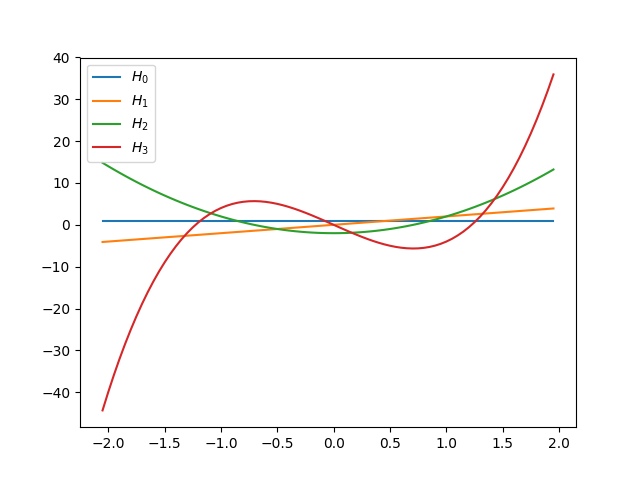
\includegraphics[scale=0.40]{learning/img/hermite_small.png} &
		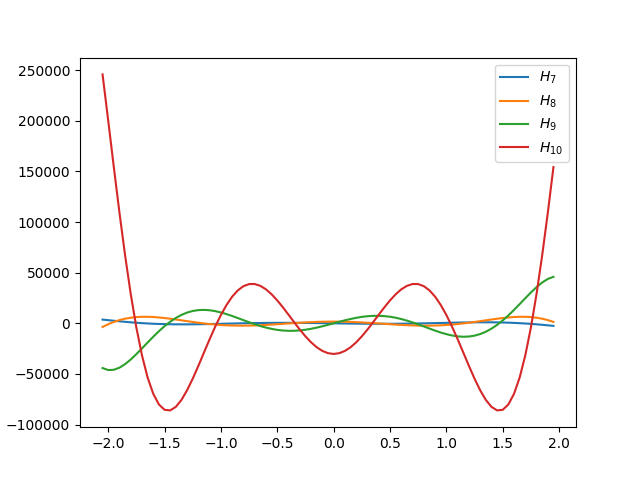
\includegraphics[scale=0.40]{learning/img/hermite_big.png} 
	\end{tabular}
	\label{fig:mst_hermite_big}
	\caption{\textbf{Links:} Die Hermite Polynome 0-ten bis 3-ten Grades \textbf{Rechts:} $H_{10}$ soll verdeutlichen wie extrem die Entwicklung zu den Rändern sich entwickelt.}
\end{figure}

\begin{figure}
	\centering
	\begin{tabular}{ccc}
		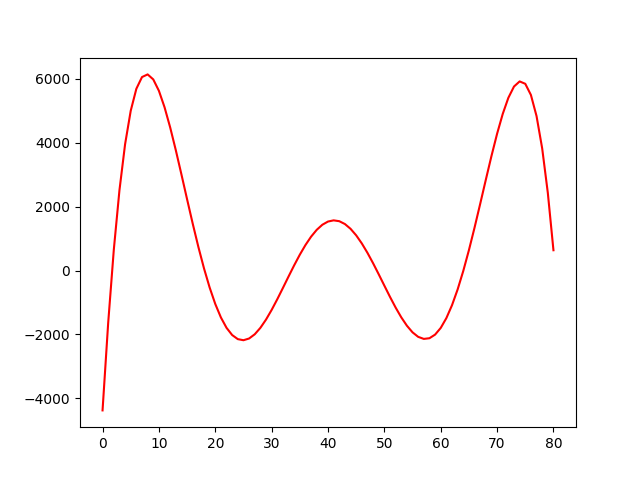
\includegraphics[scale=0.25]{learning/img/curves/wave0.png} &
		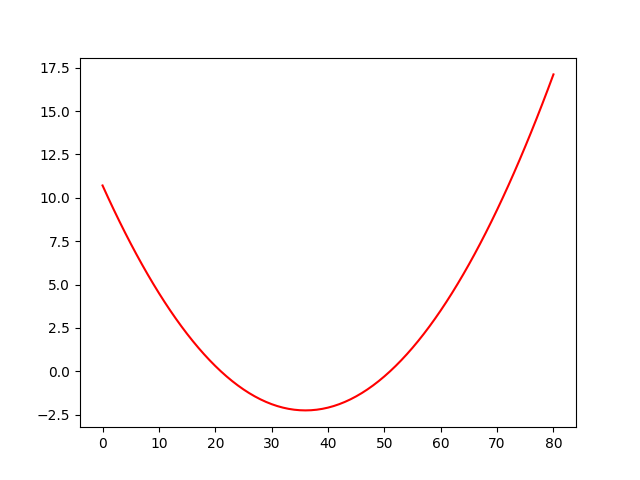
\includegraphics[scale=0.25]{learning/img/curves/wave1.png} &
		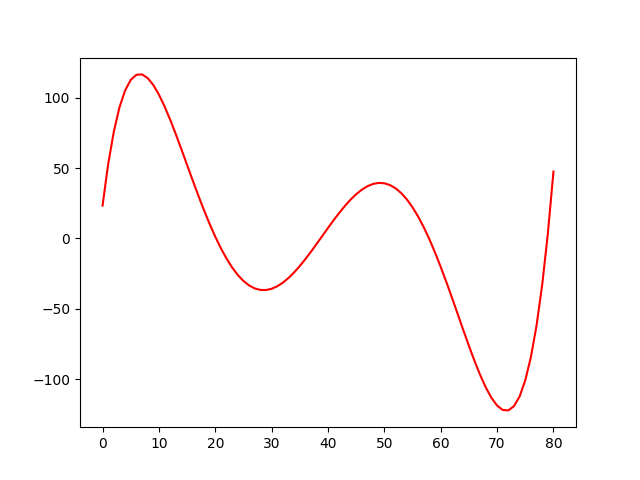
\includegraphics[scale=0.25]{learning/img/curves/wave2.png} \\
		
		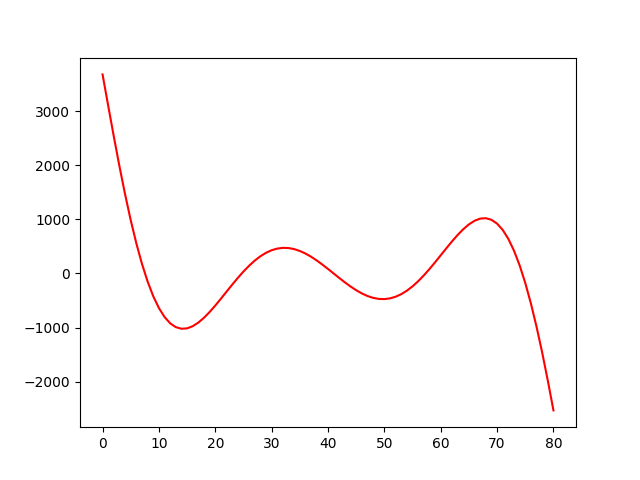
\includegraphics[scale=0.25]{learning/img/curves/wave8.png} &
		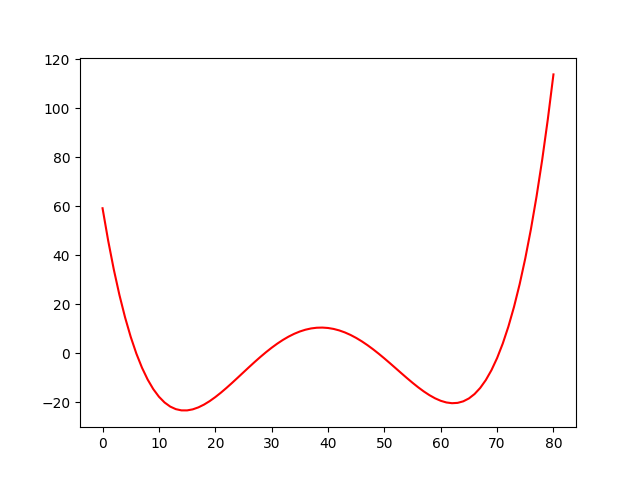
\includegraphics[scale=0.25]{learning/img/curves/wave4.png} &
		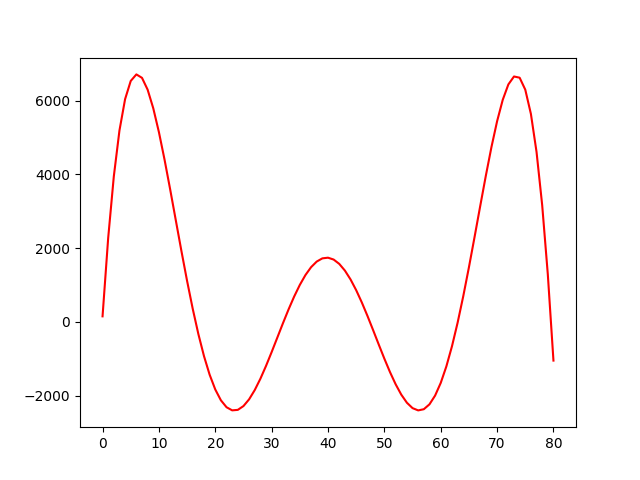
\includegraphics[scale=0.25]{learning/img/curves/wave3.png}
	\end{tabular}
	\label{fig:mst_hermiteexample}
	\caption{Einige Beispiele von Kurven die Mittels Hermite-Polynom erzeugt wurden.}
\end{figure}

Aus den generierten Kurven werden mithilfe eines ODE-Solvers die Input und Output Daten erzeugt. Die Kurven werden diskretisiert und aus Form-Gründen in die Vektoren $I_n$ und $O_n$ aufgeteilt. Die Diskretisierung erfolt auf dem Interval [-2.05, 2) mit einem Abstand von 0.05, dies resultiert in 80 Punkten, welche zu Input Vektoren konvertiert werden. Es werden pro Kurve mehrere Vektorpaare gebildet um die Daten so gut wie möglich auszunutzen. Mihilfe dieser Daten wird nun das Neuronale Netzwerk trainiert.

\subsection{Resultate}
Nach zahlreichen Trainingsanläufen mit unzähligen Iterationen kann festgehalten werden, dass die mathematische Herleitung genau dem Erlernten des Neuronalen Netzwerks entspricht (vgl. Tabelle \ref{tbl:result_heat}) Das Tabelle enthält nur ein Beispiel welches aus dem Training hergeleitet werden konnte. Die Resultate sind nicht deterministisch, da die Generierung der Daten randomisiert stattgefunden hat. Wichtig ist aber, dass die Lösungsform ($w = \xi \cdot (1, -2, 1)$) stets erfüllt wurde.

\begin{table}
	\centering
	\def\arraystretch{1.1}
	\begin{tabular}{l|c|c}
		Parameter & Erwartung & Experiment \\
		\hline
		$w$ & $\xi \cdot \begin{bmatrix} 1 \\ -2 \\ 1 \end{bmatrix}$ & $\begin{bmatrix} 0.36 \\ -0.73 \\ 0.37 \end{bmatrix}$ \\
		$b$ & 0 & 0 \\
	\end{tabular}
	\label{tbl:result_heat}
	\caption{Resultate der erlernten Wärmeleitungsgleichung.}
\end{table}

Es wurde mit einem einfachen Experiment gezeigt, dass das Lernverhalten des neuronalen Netzwerkes anhand eines einfachen Beispiels verstanden werden kann und durchaus durchschaubar ist. Das Problem dieses Beispiels ist jedoch, dass ein KNN nicht wirklich benötigt wird, da im Grunde die Lösung numerisch einfach bestimmt werden kann.